% Options for packages loaded elsewhere
\PassOptionsToPackage{unicode}{hyperref}
\PassOptionsToPackage{hyphens}{url}
%
\documentclass[
]{article}
\usepackage{amsmath,amssymb}
\usepackage{iftex}
\ifPDFTeX
  \usepackage[T1]{fontenc}
  \usepackage[utf8]{inputenc}
  \usepackage{textcomp} % provide euro and other symbols
\else % if luatex or xetex
  \usepackage{unicode-math} % this also loads fontspec
  \defaultfontfeatures{Scale=MatchLowercase}
  \defaultfontfeatures[\rmfamily]{Ligatures=TeX,Scale=1}
\fi
\usepackage{lmodern}
\ifPDFTeX\else
  % xetex/luatex font selection
\fi
% Use upquote if available, for straight quotes in verbatim environments
\IfFileExists{upquote.sty}{\usepackage{upquote}}{}
\IfFileExists{microtype.sty}{% use microtype if available
  \usepackage[]{microtype}
  \UseMicrotypeSet[protrusion]{basicmath} % disable protrusion for tt fonts
}{}
\makeatletter
\@ifundefined{KOMAClassName}{% if non-KOMA class
  \IfFileExists{parskip.sty}{%
    \usepackage{parskip}
  }{% else
    \setlength{\parindent}{0pt}
    \setlength{\parskip}{6pt plus 2pt minus 1pt}}
}{% if KOMA class
  \KOMAoptions{parskip=half}}
\makeatother
\usepackage{xcolor}
\usepackage[margin=1in]{geometry}
\usepackage{longtable,booktabs,array}
\usepackage{calc} % for calculating minipage widths
% Correct order of tables after \paragraph or \subparagraph
\usepackage{etoolbox}
\makeatletter
\patchcmd\longtable{\par}{\if@noskipsec\mbox{}\fi\par}{}{}
\makeatother
% Allow footnotes in longtable head/foot
\IfFileExists{footnotehyper.sty}{\usepackage{footnotehyper}}{\usepackage{footnote}}
\makesavenoteenv{longtable}
\usepackage{graphicx}
\makeatletter
\def\maxwidth{\ifdim\Gin@nat@width>\linewidth\linewidth\else\Gin@nat@width\fi}
\def\maxheight{\ifdim\Gin@nat@height>\textheight\textheight\else\Gin@nat@height\fi}
\makeatother
% Scale images if necessary, so that they will not overflow the page
% margins by default, and it is still possible to overwrite the defaults
% using explicit options in \includegraphics[width, height, ...]{}
\setkeys{Gin}{width=\maxwidth,height=\maxheight,keepaspectratio}
% Set default figure placement to htbp
\makeatletter
\def\fps@figure{htbp}
\makeatother
\setlength{\emergencystretch}{3em} % prevent overfull lines
\providecommand{\tightlist}{%
  \setlength{\itemsep}{0pt}\setlength{\parskip}{0pt}}
\setcounter{secnumdepth}{5}
% definitions for citeproc citations
\NewDocumentCommand\citeproctext{}{}
\NewDocumentCommand\citeproc{mm}{%
  \begingroup\def\citeproctext{#2}\cite{#1}\endgroup}
\makeatletter
 % allow citations to break across lines
 \let\@cite@ofmt\@firstofone
 % avoid brackets around text for \cite:
 \def\@biblabel#1{}
 \def\@cite#1#2{{#1\if@tempswa , #2\fi}}
\makeatother
\newlength{\cslhangindent}
\setlength{\cslhangindent}{1.5em}
\newlength{\csllabelwidth}
\setlength{\csllabelwidth}{3em}
\newenvironment{CSLReferences}[2] % #1 hanging-indent, #2 entry-spacing
 {\begin{list}{}{%
  \setlength{\itemindent}{0pt}
  \setlength{\leftmargin}{0pt}
  \setlength{\parsep}{0pt}
  % turn on hanging indent if param 1 is 1
  \ifodd #1
   \setlength{\leftmargin}{\cslhangindent}
   \setlength{\itemindent}{-1\cslhangindent}
  \fi
  % set entry spacing
  \setlength{\itemsep}{#2\baselineskip}}}
 {\end{list}}
\usepackage{calc}
\newcommand{\CSLBlock}[1]{\hfill\break\parbox[t]{\linewidth}{\strut\ignorespaces#1\strut}}
\newcommand{\CSLLeftMargin}[1]{\parbox[t]{\csllabelwidth}{\strut#1\strut}}
\newcommand{\CSLRightInline}[1]{\parbox[t]{\linewidth - \csllabelwidth}{\strut#1\strut}}
\newcommand{\CSLIndent}[1]{\hspace{\cslhangindent}#1}
\ifLuaTeX
  \usepackage{selnolig}  % disable illegal ligatures
\fi
\usepackage{bookmark}
\IfFileExists{xurl.sty}{\usepackage{xurl}}{} % add URL line breaks if available
\urlstyle{same}
\hypersetup{
  pdftitle={Linear Regression},
  pdfauthor={Walter Gruber},
  hidelinks,
  pdfcreator={LaTeX via pandoc}}

\title{Linear Regression}
\author{Walter Gruber}
\date{2025-03-13}

\begin{document}
\maketitle

{
\setcounter{tocdepth}{2}
\tableofcontents
}
\section*{}\label{section}
\addcontentsline{toc}{section}{}

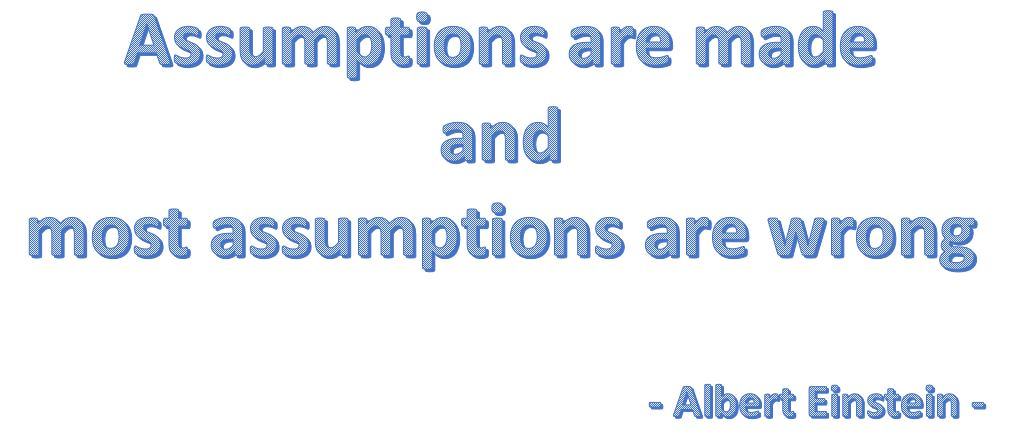
\includegraphics[width=1\textwidth,height=\textheight]{Images/Assumptions.JPG}

\section*{Vorwort}\label{vorwort}
\addcontentsline{toc}{section}{Vorwort}

This summary of robust methods is (mainly) based on an articles of Andy Field and Rand Wilcox (\citeproc{ref-FieldWilcox.2017}{Field 2017}), David Erceg-Hurn et.al. (\citeproc{ref-Hurn.2008}{Hurn 2008}), Mair (\citeproc{ref-Mair.2020}{Mair 2020}) and Wilcox (\citeproc{ref-Wilcox.2012}{Wilcox 2012}). Parts of the texts from the papers and books mentioned above have been included unchanged to this summary.

\section*{Einführung in die Einfache Lineare Regression}\label{einfuxfchrung-in-die-einfache-lineare-regression}
\addcontentsline{toc}{section}{Einführung in die Einfache Lineare Regression}

In einer Welt, die zunehmend von Daten geprägt ist, sind statistische Methoden unverzichtbare Werkzeuge, um Muster aufzudecken und fundierte Entscheidungen zu treffen. Die einfache lineare Regression ist eine der grundlegendsten, aber zugleich wirkungsvollsten Techniken in der Statistik. Sie ermöglicht es, den Zusammenhang zwischen zwei quantitativen Variablen zu modellieren und vorherzusagen, wie sich Änderungen in einer unabhängigen Variable auf eine abhängige Variable auswirken.

In diesem Kapitel werden wir die Grundlagen der einfachen linearen Regression erkunden:

\begin{itemize}
\tightlist
\item
  Was bedeutet es, einen linearen Zusammenhang zwischen zwei Variablen zu postulieren?
\item
  Wie wird ein lineares Regressionsmodell aufgestellt und interpretiert?
\item
  Durch anschauliche Beispiele und Schritt-für-Schritt-Anleitungen werden wir die Schlüsselkonzepte und mathematischen Grundlagen dieser Methode erläutern.
\end{itemize}

Ziel ist es, Ihnen ein solides Verständnis für die einfache lineare Regression zu vermitteln, das als Basis für komplexere statistische Analysen dient.

\phantomsection\label{refs}
\begin{CSLReferences}{1}{0}
\bibitem[\citeproctext]{ref-FieldWilcox.2017}
Field, \& Wilcox, A. P. 2017. {``Robust Statistical Methods: A Primer for Clinical Psychology and Experimental Psychopathology Researchers.''} \emph{Behaviour Research and Therapy, 98, 19-38}. https://doi.org/\url{https://doi.org/10.1016/j.brat.2017.05.013}.

\bibitem[\citeproctext]{ref-Hurn.2008}
Hurn, M. David. 2008. {``Modern Robust Statistical Methods: An Easy Way to Maximize the Accuracy and Power of Your Research.''} \emph{American Psychologist, Vol. 63, No. 7, 591--601}. \url{https://doi.org/10.1037/0003-066X.63.7.591}.

\bibitem[\citeproctext]{ref-Mair.2020}
Mair, Wilcox R., P. 2020. {``Robust Statistical Methods in r Using the WRS2 Package.''} \emph{Behavioural Research Methods, 52(2), 464-488}. \url{https://doi.org/10.3758/s13428-019-01246-w}.

\bibitem[\citeproctext]{ref-Wilcox.2012}
Wilcox, R. 2012. \emph{Introduction to Robust Estimation \& Hypothesis Testing.} 3rd ed. Amsterdam, The Netherlands: {Elsevier}.

\end{CSLReferences}

\end{document}
